% Experiment 4b only. Do not \input this from the paper until the label is agreed.
% Suggested label: fig:exp4b-beta. Do not reuse fig:exp4-full.
% The PDF is exactly 178 mm wide. This fragment is not a standalone display document.
\begin{figure*}[t]
  \centering
  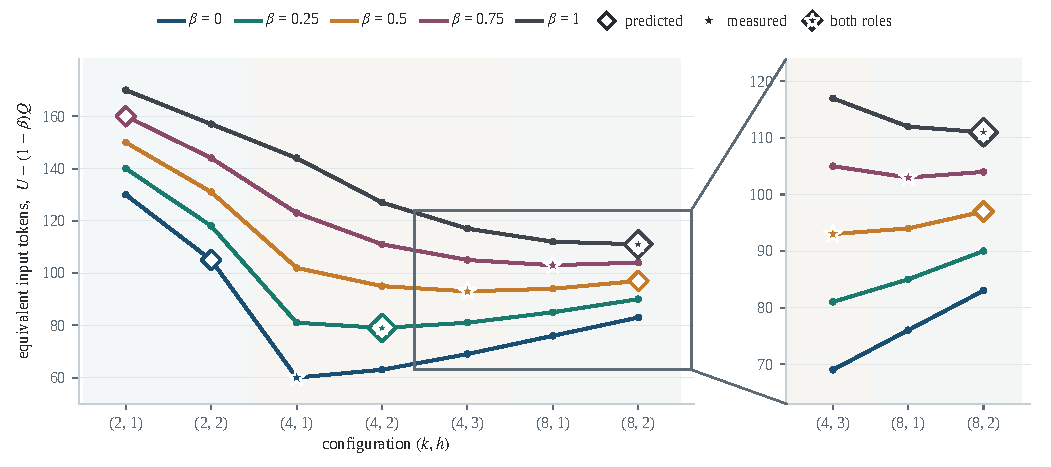
\includegraphics[width=178mm]{e4b-beta.pdf}
  \caption{Synthetic layout sample for offline $\beta$ repricing of one invented On-cold observation.
  These tokens are not a measurement, and the figure supports no conclusion.
  Five curves show $U-(1-\beta)Q$ for $\beta = 0$, $0.25$, $0.5$, $0.75$, and $1$
  on one shared categorical $(k,h)$ axis, displayed in $k$-then-$h$ order.
  The segments join those configurations; the axis is not a continuous $(k,h)$ scale.
  $\beta = 1$ stays cache-on and applies no hit discount.
  A diamond is the predicted configuration and a star is the measured minimum of that curve.
  Both marks are drawn at the measured cost of the marked configuration.
  A star on a diamond means the two roles fall on the same configuration.
  The right panel repeats the framed categories with the same labels.
  Contract values $\beta = 0.1$ and $0.9$ are not drawn.}
  \label{fig:exp4b-beta}
\end{figure*}
